
%(BEGIN_QUESTION)
% Copyright 2014, Tony R. Kuphaldt, released under the Creative Commons Attribution License (v 1.0)
% This means you may do almost anything with this work of mine, so long as you give me proper credit

Suppose you ran a ``scan'' diagnostic test on a globe-style control valve equipped with a DVC6200 positioner, and obtained the following {\it valve signature} plot:

$$\includegraphics[width=15.5cm]{i02148x01.eps}$$

First, identify the problem revealed by the signature plot.  Next, identify what would have to be done to the valve to correct this problem.

\underbar{file i02148}
%(END_QUESTION)





%(BEGIN_ANSWER)

Half-credit for properly identifying the problem, half credit for a correct fix.

\vskip 10pt

The problem with this valve is at the lower end, where the plug contacts the seat.  There is clearly some mechanical interference occuring at this point, as revealed by the sharp rise in pressure necessary to make the plug lift off the seat while opening as well as the gradual drop-off of pressure as the plug re-seats while closing.

\vskip 10pt

The only proper fix for this is to replace the damaged trim components so that they fit together properly.

%(END_ANSWER)





%(BEGIN_NOTES)

{\bf This question is intended for exams only and not worksheets!}.

%(END_NOTES)


